\begin{chapter}{Topología de $\mathbb{R}^n$}
En esta sección se estudian conceptos relacionados con la topología de $\mathbb{R}^n$, con particular énfasis en la definición de abiertos, vecindades, ...

\begin{section}{Conjuntos abiertos y cerrados}

En esta sección se desarrollará lo básico sobre la topología estándar del espacio euclidiano. Se trabajará entonces sobre el conjunto $\mathbb{R}^n$ con su estructura usual de espacio vectorial. Empecemos primero por las nociones básicas que dan lugar a la estructura de abiertos que requerimos.

\begin{defn}

Una norma en $\mathbb{R}^n$ es una función $|\cdot|: \mathbb{R}^n \to \mathbb{R}$ que cumple las siguientes condiciones.

\begin{enumerate}
    \item para todo $a\in \mathbb{R}^n$ se cumple $|a| \geq 0$, donde la igualdad se da si y sólo si $a = 0$.
    \item para cualquier número real $\alpha$ y $a \in \mathbb{R}^n$ se tiene $|\alpha a| = |\alpha| |a|$.
    \item Para cualquier par de vectores $a,b \in \mathbb{R}^n$ se tiene $|a+b| \leq |a| + |b|$.
\end{enumerate}

\end{defn}

Notese que en la segunda propiedad se abusa ligeramente de la notación al denotar por $|\cdot|$ tanto el valor absoluto en la recta como la norma en cuestión que se está definiendo.  

Algunos ejemplos clásicos de normas en $\mathbb{R}^n$ son los siguientes, para $a = a^{\mu} e_{\mu}$, donde $\{ e_{\mu} \}$ representa la base estándar de $\mathbb{R}^n$ y se está asumiendo la convención de suma de Einstein.
$$|a| = \sum_{j} |a^{j}|, \ |a| = \max_{i} |a^i|, \ |a| = \sum_j (a^j)^2\,.$$
Las tres funciones anteriores definen normas, estas se llaman respectivamente norma de la suma, norma del máximo y norma euclidiana. 

Pasamos ahora a definir lo que son las bolas determinadas por una norma.

\begin{defn}

Dada una norma $|.|$ en $\mathbb{R}^n$ y $\epsilon > 0$ se define la bola abierta centrada en $a \in \mathbb{R}^n$, con radio $\epsilon$ como
$$B(a,\epsilon) = \{ v \in \mathbb{R}^n : |a - v|< \epsilon  \}\,.$$

\end{defn}

Las nociones de bola cerrada $B[a, \epsilon]$ y esfera $S[a, \epsilon]$ se definen de forma análoga cambiando la desigualdad por una de tipo menor o igual y por una igualdad. Se puede observar que la forma geométrica de las bolas depende de la norma escogida. Sin embargo, el concepto definido a continuación si resulta independiente de la norma.

\begin{defn}

Un subconjunto $U \subset \mathbb{R}^n$ se llama abierto cuando para cualquier $x \in U$ existe $\epsilon > 0$ tal que $B(x, \epsilon) \subset U$.

\end{defn}

De manera análoga se puede definir un abierto como un conjunto que es igual a su interior, donde el interior $\text{int}(A)$ es todos los puntos de $A$ que verifican la existencia de una bola como en la definición anterior.

El siguiente resultado, que se enunciará sin probar, confirma el hecho de que la definición de abierto no depende de la norma escogida.

\begin{them}

Dado cualquier par de normas $|.|_1$ y $|.|_2$ en $\mathbb{R}^n$, existen $C_1, C_2 > 0$ tales que
$$C_1|a|_1 \leq |a|_2 \leq C_2|a|_1\,.$$

\end{them}  

De esta forma resulta evidente la invarianza del concepto de abierto, pues por medio de la existencia de estas constantes uno puede siempre encajar una bola de cierta norma dentro de una de cualquier otra norma. La estructura de abiertos de $\mathbb{R}^n$ le da a este espacio una estructura de espacio topológico. Esto es

\begin{them}

Los abiertos en $\mathbb{R}^n$ cumplen las siguientes propiedades.

\begin{enumerate}
    \item $\mathbb{R}^n$ y $\emptyset$ son abiertos.
    \item La intersección de una familia finita de abiertos da como resultado un conjunto abierto.
    \item La intersección de una familia arbitraria de abiertos da como resultado un conjunto abierto.
\end{enumerate}

\end{them}

El hecho de que la definición de abierto no dependa de la norma escogida se puede afirmar de manera condensada diciendo que todas las normas en $\mathbb{R}^n$ inducen la misma topología.

Pasemos ahora a hablar brevemente de lo que es un conjunto cerrado y enunciar un teorema análogo al anterior.

\begin{defn}

$F \subset \mathbb{R}^n$ es llamado conjunto cerrado, cuando su complemento es abierto.

\end{defn}

\begin{them}

Los conjuntos cerrados gozan de las siguientes propiedades.

\begin{enumerate}
    \item $\mathbb{R}^n$ y $\emptyset$ son cerrados.
    \item La unión de una familia finita de cerrados es un cerrado.
    \item La intersección de una familia arbitraria de cerrados es un cerrado.
\end{enumerate}
\end{them}

Antes de continuar, y con el fin de hacer algunos conceptos futuros más sencillos, se definirá que un abierto $U_A$ de un subconjunto $A \subset \mathbb{R}^n$ como la intersección de un abierto de $\mathbb{R}^n$ con el propio $A$. Esto es, los abiertos de $A$ son todos de la forma $U \cap A$ donde $U$ es un abierto de $\mathbb{R}^n$. De manera análoga se define lo que es un cerrado en $A$.

\begin{defn}[Punto de acumulación]
Se dice que un punto $a \in \R^n$ es un punto de acumulación de un conjunto $A \subset R^n$, cuando toda bola abierta de $A$ centrada en $a$ contiene algún punto de $A$ diferente de $a$, en otras palabras, para todo numero real $\epsilon > 0$ se tiene que $A \cap B(a, \epsilon) \setminus \{a\} \neq \emptyset$
\end{defn}

\begin{notn}
El conjunto de puntos de acumulación de un conjunto $A$ se denotara por A'.
\end{notn}

\begin{exer}
Dado un conjunto $A$, las siguientes afirmaciones son equivalentes:
\begin{enumerate}
\item $a \in A'$.
\item Existe $\{a_n\}_{n \in \N}$ con $a_i \in A$ para algún $i \in \N$, tal que $\{a_n\} \to a$.
\item Toda bola abierta centrada en $a$ contiene infinitos puntos de $A$.
\end{enumerate}
\end{exer}

\begin{defn}
Se dice que un punto $a \in \R^n$ es un punto de adherencia de un conjunto $A$, si para toda bola abierta (vecindad) centrada en $a$ (de $A$) de radio $\epsilon \in \R$ con $\epsilon > 0$, se cumple que $A \cap B(a, \epsilon) \neq \emptyset$
\end{defn}

\begin{notn}
El conjunto de puntos de adherencia de un conjunto $X$ se denotara por $\bar{X}$
\end{notn}

Le definición anterior es útil porque da caracterización adicional de cuando un conjunto es cerrado, esto es, se dice que un conjunto $X \subset \R^n$ es cerrado si y solo si $X = \bar{X}$. Además de esta, el siguiente ejercicio muestra otra caracterización de conjuntos cerrados.

\begin{exer}
Un conjunto $X \subset \R^n$ es cerrado si y solo si $X^c \subseteq_{op} \R^n$.
\end{exer}

\end{section}

\begin{section}{Convergencia de sucesiones y continuidad de aplicaciones}

Una sucesión en $\mathbb{R}^n$ se define como una aplicación $\phi: \mathbb{N} \to \mathbb{R}^n$. Usualmente se denota la sucesión como su conjunto de valores, es decir, $( \phi(n))_{n \in \mathbb{N}}$, o también $(\phi_n)_{n \geq 1}$. Una subsucesión de $\{ \phi_n \}$ se obtiene a partir de una función creciente con imagen infinita $i: \mathbb{N} \to \mathbb{N}$. De esta forma, a la sucesión $\phi \circ i$ se le llama subsucesión de $(\phi_n )$, usualmente denotada $( \phi_{i(n)} )$. A continuación nos enfocamos en hablar sobre convergencia de sucesiones.

\begin{defn}

Decimos que la sucesión $(a_n)$ con $a_n \in \mathbb{R}^n$ converge a $a \in \mathbb{R}^n$ cuando $\forall \epsilon > 0$ $\exists N \in \mathbb{N}$ tal que $n > N \Rightarrow |a_n - a| < \epsilon$. En simbolos esto se denota como $(a_n) \to a$.

\end{defn}

La definición anterior no depende de la norma escogida, lo cual es consecuencia de que en un espacio euclidiano todas las normas inducen la misma topología. La definición anterior se puede enunciar en términos de bolas de la siguiente forma

$$(a_n) \to a  \iff \forall \epsilon > 0 \exists N \in \mathbb{N} \ \text{tal que} \ n>N \Rightarrow a_n \in B(a,\epsilon)\,.$$

Más aún, se puede hacer en términos de abiertos. Si entendemos por vecindad en $\mathbb{R}^n$ de $a$, a cualquier abierto $U$ de $\mathbb{R}^n$, que contiene a $a$. Más aún, denotando por $N_a$ a la familia de todas las vecindades de $a$ en $\mathbb{R}^n$, entonces
$$(a_n) \to a \iff \forall U \in N_a \exists N \in \mathbb{N} \ \text{tal que} \ n>N \Rightarrow a_n \in U\,.$$
La definición anterior goza de ser independiente de la estructura métrica de $\mathbb{R}^n$. Por lo tanto puede ser adoptada para hablar de convergencia en cualquier espacio topológico.

El siguiente teorema, que resulta intuitivo en $\mathbb{R}^n$, no es cierto en cualquier espacio topológico, de hecho, depende crucialmente de que cualquier par de puntos distintos tengan vecindades disjuntas. Lo anterior, que es evidente en un espacio euclidiano, se conoce como propiedad de Hausdorff, y los espacios topológicos que la cumplen se denominan espacios topológicos Hausdorff.

\begin{them}

El límite de una sucesión convergente en $\mathbb{R}^n$ es único.

\end{them}

\begin{proof}

Supongamos que $(a_n)$ converge a dos puntos distintos $x, y \in \mathbb{R}^n$. Tomando las bolas $B(x,\epsilon)$, $B(y, \epsilon)$, con $\epsilon$ suficientemente pequeño, de tal forma que estas bolas sean disjuntas, se obtiene una contradicción al suponer que la sucesión converge a ambos puntos. Para entender esta contradicción, veáse la definición de convergencia en términos de bolas. El epsilon puede tomarse por ejemplo, como menor a $\frac{|x-y|}{2}$.

\end{proof}

Las propiedades básicas sobre convergencia de sucesiones se dejan al lector (suma de sucesiones convergentes es convergente, producto por un escalar, producto punto, etc.). Se puede consultar \cite{lima2004curso} para ver estas propiedades con más detalle.

Ahora bien, entiéndase por aplicación a una función $f: A \subset \mathbb{R}^n \ to \mathbb{R}^m$. Se estudiará a continuación el concepto de continuidad de una aplicación. Sin embargo, antes de esto, definamos brevemente lo que es un límite. 

\begin{defn}

Sea $f: A\subset \mathbb{R}^n \to \mathbb{R}^m$. Dadas normas $|.|_1$ y $|.|_2$ en $\mathbb{R}^n$ y $\mathbb{R}^m$, decimos que
$$\lim_{x \to a} f(x) = b\,,$$
cuando
$$\forall \epsilon > 0 \exists \delta > 0 \ \text{tal que} \ |x-a|_1 < \delta \Rightarrow |f(x) - b|_2 < \epsilon\,.$$
Queda como ejercicio para el lector reescribir la definición anterior en términos de bolas y en términos de abiertos, como se hizo para la convergencia de una sucesión. Además de esto, por el hecho de que todas las normas inducen la misma topología, la definición anterior no depende de las normas escogidas.  

\end{defn}



\begin{defn}
Una aplicación $f: X \subset \R^n \to \R^m$ se dice continua en un punto $p \in X$, si para todo $\epsilon > 0$ existe $\delta > 0$ tal que si para $x \in X$ $|x - p| < \delta$ implica que $|f(x) - f(p)| < \epsilon$ con $\epsilon, \delta \in \R$.
\end{defn}

\begin{rem}
Por la definición anterior, la continuidad de $f: X \subset \R^n \to \R^m$ esta totalmente garantizada si para todo $\epsilon > 0$ existe $\delta > 0$ tal que $x \in X \cap B(p, \delta)$ implica que $f(x) \in B(f(p), \epsilon)$ con $\epsilon, \delta \in \R$.
\end{rem}

\begin{exer}
Demostrar que la continuidad de una funcion esta caracterizada por la siguiente afirmacion. Una funcion $f: X \subset \R^n \to \R^m$ es continua, si para cualquier secuencia $(x_n)_{n \in \N} \subseteq X$ que converge a un punto $x \in X$, entonces la secuencia $(f(x_n))_{n \in \N}$ converge a $f(x)$.
\end{exer}

\begin{defn}
Se dice que una funcion $f: X \subset \R^n \to \R^m$ es Lipchitziana cuando existe $k \in \R$ con $k > 0$ tal que $|f(x) - f(y)| < k|x - y|$.
\end{defn}

\begin{lema}
Toda aplicación Lipchitziana es continua
\end{lema}

\end{section}

\begin{section}{Compacidad}
Antes de dar la definición de compacidad, motívese esta a través de una visualización debida a John D. Baum: 

\begin{quote}
    Supongamos que una gran multitud de personas --posiblemente infinitas-- están afuera bajo la lluvia, y que cada una de estas personas usa su sombrilla, claramente ellas permanecerán sin mojarse. Pero por supuesto es posible que ellas estén juntas de manera tan compacta, que no sea necesario sino que un número finito de ellas abran sus sombrillas y todavía permanezcan sin mojarse. En este caso pensamos que ellas forman una especie de espacio compacto
\end{quote}

\begin{defn}
Sea $X$ un E.T. Se dice que $X$ es compacto, si dado un cubrimiento de abiertos de $X$, i.e. una colección $\{\mathcal{U}_\alpha\}$ de abiertos de $X$ t.q. $X\subseteq\bigcup\mathcal{U}_\alpha$, existe un subcubrimiento finito que también cubre a $X$, i.e. una subcolección $\{\mathcal{U}_{\alpha(i)}\}_{i=1}^n\subseteq\{\mathcal{U}_\alpha\}$ t.q. $X\subseteq\bigcup_{i=1}^n\mathcal{U}_{\alpha(i)}$. Adicionalmente, si $Y\subseteq X$, se dice que $Y$ es compacto si es compacto con la topología relativa.
\end{defn}

La propiedad de ser compacto, a diferencia de ser abierto o cerrado, no depende de las características del espacio en donde estén sumergidos los conjuntos, i.e. que es una característica absoluta, no relativa, pues existen E.T. donde se pueden tener conjuntos $X\subseteq Y\subseteq Z$, t.q. $X$ sea abierto relativo en $Y$, sin serlo en $X$. Por ejemplo, considérese $Z=\R$ con la topología usual. Si $X=]0.5,1]$ y $Y=[0,1]$, nótese que $X=]0.5,2[\cap Y$, i.e. que $X$ es abierto relativo en $Y$, pero claramente no lo es en $Z$. Demuéstrese a continuación lo dicho:

\begin{them}
Supóngase que $X\subseteq Y\subseteq Z$. Se tiene que $X$ es compacto relativo en $Z$ syss $X$ es compacto relativo en $Y$.
\end{them}

\begin{proof}
Sea $X$ compacto relativo en $Z$ y sea $\{\mathcal{U}_\alpha\}$ una colección de conjuntos abiertos relativos en $Y$ t.q. $X\subseteq\bigcup\mathcal{U}_\alpha=\bigcup\left(\mathcal{V}_\alpha\cap Y\right)$, donde para cada $\alpha$, $\mathcal{V}_\alpha$ es abierto de $Z$. En particular se tiene que $X\subseteq\mathcal{V}_{\alpha(1)}\cup\cdots\cup\mathcal{V}_{\alpha(n)}$, i.e. que $X=X \cap Y\subseteq(\mathcal{V}_{\alpha(1)}\cup\cdots\cup\mathcal{V}_{\alpha(n)})\cap Y=(\mathcal{V}_{\alpha(1)}\cap Y)\cup\cdots\cup(\mathcal{V}_{\alpha(n)}\cap Y)=\mathcal{U}_{\alpha(1)}\cup\cdots\cup\mathcal{U}_{\alpha(n)}$, i.e. que $X$ es compacto relativo en $Y$.

Finalmente, si se supone $X$ compacto relativo en $Y$ y $\{\mathcal{V}_\alpha\}$ una colección de abiertos de $Z$ que cubre a $X$, defínase $\mathcal{U}_\alpha:=\mathcal{V}_\alpha\cap Y$, luego $X\subseteq\mathcal{U}_{\alpha(1)}\cup\cdots\cup\mathcal{U}_{\alpha(n)}$, pero como para toda $\alpha$, $\mathcal{U}_\alpha\subseteq\mathcal{V}_\alpha$, claramente $X\subseteq\mathcal{V}_{\alpha(1)}\cup\cdots\cup\mathcal{V}_{\alpha(n)}$, i.e. que $X$ es compacto relativo en $Z$.
\end{proof}

En virtud del teorema anterior se puede, en muchos casos, considerar conjuntos compactos como E.T. en sí mismos, sin prestar atención al espacio que los contiene. En particular, aunque tiene escaso sentido hablar de espacios abiertos o cerrados (pues todo E.T. es en sí mismo tanto abierto como cerrado), sí tiene sentido hablar de E.T. compactos. 

\begin{exmp}
Es claro que cualquier conjunto finito de un E.T. es compacto.
\end{exmp}

\begin{exmp}
Los intervalos cerrados de $\mathbb{R}$ son compactos.

Supóngase el intervalo $[a,b]$ t.q. $a<b$, pues si $a=b$ el resultado es trivial. Considérese una colección de abiertos $\{\mathcal{U}_j\}_{j\in J}$ de $[a,b]$, que cubren tal intervalo, donde $\mathcal{U}_j=\mathcal{V}_j\cap[a,b]$, con $\mathcal{V}_j$ abierto de $\R$, para toda $j$. Defínase el conjunto: $$S:=\left\lbrace x\in[a,b]:[a,x]\subseteq\bigcup_{j\in I\subseteq J}\mathcal{U}_j\wedge|I|<\aleph_0\right\rbrace.$$ Es claro que $a\in S$, i.e. que $S\neq\emptyset$. Además, si $c\in S$, entonces $[a,c]\subseteq S$. Según lo anterior, por el principio del supremo, como también $S$ está acotado superiormente por $b$, existe $d=\sup(S)$.
\end{exmp}

\begin{rem}
Nótese que si una colección $\{\mathcal{U}_\alpha\}$ de conjuntos de $X$, recubre a $X$, i.e. que $X\subseteq\bigcup\mathcal{U}_\alpha$, entonces $X=\bigcup\mathcal{U}_\alpha$. Luego, en la definición anterior es indiferente decir si el recubrimiento de abiertos contiene al conjunto o es igual a éste. 
\end{rem}

\begin{them}
Sea $X$ un E.T. compacto y $Y\subseteq X$ cerrado, entonces $Y$ es compacto. 
\end{them}

\begin{proof}
Sea $\{\mathcal{U}_\alpha\}$ un cubrimiento de abiertos para $Y$. Como $Y$ es cerrado en $X$, por definición $Y^C=X-Y$ es abierto en $X$. Nótese que si $Y^C=\emptyset$, entonces $Y=X$ y trivialmente sería compacto, así que supóngase $Y^C\neq\emptyset$. Nótese que:
\begin{equation*} \label{eq1}
\begin{split}
X & = Y^C\cup Y \\
 & = Y^C\cup\bigcup\mathcal{U}_\alpha \\
 & = Y^C\cup\bigcup\underbrace{(Y\cap\mathcal{V}_\alpha)}_{\text{abiertos de $Y$}} \\
 & = Y^C\cup \left(Y\cap\bigcup\mathcal{V}_\alpha\right) \\
 & = (Y^C\cup Y)\cap \left(Y^C\cup\bigcup\mathcal{V}_\alpha\right) \\
 & = X\cup\left(Y^C\cup\bigcup\mathcal{V}_\alpha\right),
\end{split}
\end{equation*}
y nótese que el conjunto resultante en la igualdad de la última linea, es un abierto de $X$, i.e. que en particular $\{\mathcal{U}_\alpha\}\cup\{Y^C\}$ es un cubrimiento de abiertos de $X$, y por la compacidad de $X$ nótese que existe un conjunto finito $\{\mathcal{U}_1,\ldots,\mathcal{U}_n\}\subseteq\{\mathcal{U}_\alpha\}$ t.q. $X=\bigcup_{i=1}^n\mathcal{U}_i\cup Y^C$ (pues como $Y=\bigcup\mathcal{U}_\alpha$ y $Y^C\neq\emptyset$, hay que considerar este último conjunto en el cubrimiento por si existen elementos que no están en el otro), pero como $Y\subseteq X$, entonces $Y\subseteq\bigcup_{i=1}^n\mathcal{U}_i\cup Y^C$, i.e. que $Y\subseteq\bigcup_{i=1}^n\mathcal{U}_i$, mostrando que en efecto $Y$ es compacto.
\end{proof}

\begin{them}
Sean $X$ y $Y$ E.T. Si $X$ es compacto y $f:X\to Y$ es una aplicación continua, entonces $f(X)$
es compacto.
\end{them}

\begin{exmp}
Demuéstrese que $\mathbb{S}^1:=\{(x,y)\in\mathbb{R}^2:x^2+y^2=1\}$ es un conjunto compacto. Basta considerar la función $f:[0,2\pi]\to\mathbb{S}^1$ t.q. $f(\theta)=(\cos(\theta),\sin(\theta))$. Por el teorema anterior $f([0,2\pi])=\mathbb{S}^1$ es compacto.
\end{exmp}

\begin{proof}
Si $\{\mathcal{U}_\alpha\}$ es un cubrimiento de abiertos para $f(X)$, entonces $f(X)\subseteq\bigcup\mathcal{U}_\alpha$, y por propiedades conjuntistas\footnote{Recordar de teoría de conjunto que dada la función $f:X\to Y$, la imagen directa de $A\subseteq X$ y la imagen inversa de $B\subseteq Y$ se definen respectivamente como:$$f(A):=\{y\in Y:\exists x\in A f(x)=y\}\text{ y }f^{-1}(B):=\{x\in X:f(x)\in B\}.$$ Además, $f(A)\subseteq B$ syss $A\subseteq f^{-1}(B)$. Finalmente, si para cada $\alpha$, $\mathcal{U}_\alpha\subseteq Y$, entonces $f^{-1}\left(\bigcup\mathcal{U}_\alpha\right)=\bigcup f^{-1}\left(\mathcal{U}_\alpha\right)$.} se tiene que esto último es equivalente a decir que $X\subseteq f^{-1}\left(\bigcup\mathcal{U}_\alpha\right)=\bigcup f^{-1}(\mathcal{U}_\alpha)$, pero como $f$ es continua, devuelve abiertos en abiertos, por tanto $\{f^{-1}(\mathcal{U}_\alpha)\}$ es un cubrimiento de abiertos para $X$, y por la compacidad de tal conjunto, existe un subconjunto $\left\lbrace f^{-1}(\mathcal{U}_{\alpha(i)}):i=1,\ldots,n\right\rbrace\subseteq\left\lbrace f^{-1}\left(\mathcal{U}_\alpha\right)\right\rbrace$ t.q. $X\subseteq\bigcup_{i=1}^nf^{-1}\left(\mathcal{U}_{\alpha(i)}\right)=f^{-1}\left(\bigcup_{i=1}^n\mathcal{U}_{\alpha(i)}\right)$, y esto último es equivalente a que $f(X)\subseteq\bigcup_{i=1}^n\mathcal{U}_{\alpha(i)}$.
\end{proof}

\begin{them}
El espacio producto $S\times T$ es compacto syss $S$ y $T$ son compactos. 
\end{them}

\begin{proof}
Ver \cite[pp. 24, 25]{abraham}.
\end{proof}

\begin{exmp}
Recordar que el toro es la superficie cerrada definida como $\mathbb{T}^2=\mathbb{S}^1\times\mathbb{S}^1$. Luego es compacto. 
\end{exmp}

\begin{rem}
El toro también se puede definir considerando la siguiente relación de equivalencia sobre $\mathbb{R}^2$: $$(a_1,a_2)\sim(b_1,b_2)\Leftrightarrow(a_1-b_1,a_2-b_2)\in\mathbb{Z}\times\mathbb{Z},$$ para definir $\mathbb{T}^2=\mathbb{R}^2/\sim$, donde los abiertos de la topología vienen dados por la colección $\left\lbrace\mathcal{U}\subseteq\mathbb{T}^2:\pi^{-1}\left(\mathcal{U}\right)\text{ es abierto de }\mathbb{R}^2\right\rbrace$. Recordar que la aplicación $\pi$ es la proyección canónica $\pi:\mathbb{R}^2\to\mathbb{T}^2$ t.q. $\pi(x)=[x]$. Esto muestra que el recíproco del teorema anterior es falso, pues $\mathbb{T}^2$ es compacto y $\mathbb{R}^2$ no (¿por qué?).
\end{rem}

\begin{them}[\textbf{de Bolzano-Weierstra{\ss}}]
Si $X$ es un E.T. compacto y Haussdorf, entonces toda sucesión convergente posee una subsucesión convergente. El recíproco es también verdadero en espacio métricos y E.T. Hausdorff segundo contables. 
\end{them}

\begin{proof}

\end{proof}

\begin{defn}
Sea $M$ un E.M. Un conjunto $A\subseteq M$ es llamado totalmente acotado si para todo $\epsilon>0$, existe un conjunto finito $\{p_1,\ldots,p_n\}\subseteq M$ t.q. $A\subseteq\bigcup_{i=1}^nD_\epsilon(p_i)$.
\end{defn}

\begin{them}
Un E.M. es compacto syss es completo y totalmente acotado.
\end{them}

\begin{proof}

\end{proof}

\begin{them}
En un E.M. los conjuntos compactos son cerrados y acotados.
\end{them}

\begin{proof}

\end{proof}

\begin{them}[\textbf{de Heine-Borel}]
En $\mathbb{R}^n$ ser compacto es equivalente a ser cerrado y acotado. 
\end{them}

\begin{proof}

\end{proof}

Por lo anterior y el teorema de Bolzano-Weierstra{\ss}, se tiene que $X\subseteq\mathbb{R}^n$ es compacto syss toda sucesión de puntos de $X$ posee una subsucesión convergente a un punto de $X$.

Es inmediato comprobar que $]0,1[\subseteq\mathbb{R}$ no es compacto, pues por el comentario anterior, nótese que $\{1/k\}_{k\geq2}\subseteq]0,1[$, pero tal sucesión converge a $0\notin]0,1[$.

\end{section}

\begin{section}{Conexidad}

El concepto de conexidad tiene un significado relacionado con el hecho de no poder ``separar'' un conjunto en dos partes. Los conceptos presentados acá están en el contexto de la topología estándar de los espacios euclidianos, pero la mayoría de estos se pueden generalizar de manera análoga a espacios topológicos más generales.

\begin{defn}
$A \subset \mathbb{R}^n$ se dice conexo cuando para cualquier pareja de abiertos disjuntos $U_1, U_2 \subset \mathbb{R}^n$ tales que $A \subset U_1 \cup U_2$, necesariamente uno de estos dos no intercepta a $A$.
\end{defn}
Equivalentemente podríamos definir este concepto diciendo que una separación de un conjunto es una escogencia de dos abiertos de este conjunto, que son disjuntos y que unen al conjunto. Una separación trivial es cuando uno de estos abiertos es el mismo conjunto y el otro es el conjunto vacío. Luego, un conjunto conexo es aquel que solo admite separaciones triviales. Recuerde que un abierto de un conjunto es la intersección de un abierto en $\mathbb{R}^n$ con el mismo conjunto.

El siguiente teorema es una caracterización bien conocida de los subconjuntos conexos de la recta (en la topología estándar).

\begin{them}
Los únicos subconjuntos conexos de la recta son los intervalos.
\end{them}

La conexidad, así como la compacidad, es una propiedad preservada por aplicaciones continuas, en efecto

\begin{them}
Si $f: X \subset \mathbb{R}^n \to \mathbb{R}^m$ es continua y $X$ es conexo, entonces $f(X)$ es conexo.
\end{them}

\begin{proof}
En efecto, si $U_1, U_2$ abiertos disjuntos de $f(X)$ unen al propio $f(X)$, por la continuidad de $f$, se tiene que $f^{-1}(U_1)$ y $f^{-1}(U_2)$ son abiertos de $X$, disjuntos y que unen a $X$, luego, por conexidad uno de los dos debe ser vacío, como consecuencia $U_1$ o $U_2$ es vacío.
\end{proof}

Juntando los dos teoremas anteriores se obtiene el teorema del valor intermedio para funciones reales de varias variables.

\begin{them}

Si $f: X \subset \mathbb{R}^n \to \mathbb{R}^m$ es continua y $y \in (f(x_1),f(x_2))$, entonces existe $x_3 \in X$ tal que $f(x_3) = y$.

\end{them}

El teorema anterior se prueba sin mucha dificultad teniendo en cuenta que por conexidad, la imagen de $f$ es un intervalo.

Otra aplicación interesante es el conocido teorema de la aduana.

\begin{them}

Si un conjunto conexo $X \subset \mathbb{R}^n$ contiene un punto $a \in A$ y otro punto $b \notin A$, para otro conjunto arbitrario $A \subset \mathbb{R}^n$, entonces $X$ contiene algún punto de la frontera de $A$.

\end{them}

\begin{proof}

Recordemos que la frontera de $A$, denotada por $\partial A$, se define como todos los puntos de $\mathbb{R}^n$ tales que toda bola centrada en ellos contiene puntos de $A$ y de su complemento, es decir, no son ni interiores ni exteriores.

Ahora, supongamos que $a$ y $b$ no son puntos frontera de $A$, caso contrario ya se tiene el resultado. Luego, se tiene que $a \in \text{int}(A)$ y $b \in \text{ext}(A)$. De esta forma, $\text{int}(A) \cap X$ y $\text{ext}(A) \cap X$ son abiertos de $X$ no vacíos y disjuntos, luego, no pueden unir a $X$ pues esto contradice la conexidad de $X$. Entonces, existe un punto de $X$ que no está en ninguno de estos abiertos, es decir, es un punto frontera de $A$.
\end{proof}

Como consecuencia se puede observar un hecho que se puede intuir de forma natural sobre curvas continuas. Si $\gamma: I \to \R^n$ es una curva continua. Donde $I$ es un intervalo de la recta. Entonces suponer que para algún conjunto $A \subset \R^n$ se cumple que la curva toma algún valor en este conjunto y otro por fuera, implica que toma un valor sobre la frontera.

Una pregunta natural es si la unión de conjuntos conexos es conexa. Intuitivamente se puede responder a esta pregunta negativamente, pues uno puede unir dos conexos disjuntos y el resultado evidentemente no será conexo. Sin embargo, la respuesta es afirmativa si no son disjuntos.

\begin{them}

Una unión arbitraria de conexos con un punto en común da como resultado un conjunto conexo.

\end{them}

\begin{proof}

En efecto, sea $\{ A_{\alpha} \}_{\alpha \in \Lambda}$ una familia de conexos en un espacio euclidiano, indexada por algún conjunto $\Lambda$ y $p \in A_{\alpha}$, para todo $\alpha \in \Lambda$.

Ahora, si $U_1, U_2$ son abiertos disjuntos de $A = \cup_{\alpha} A_{\alpha}$, que unen a $A$, entonces, $p \in U_1$, sin pérdida de generalidad. Luego, $U_1 \cap A_{\alpha} \neq \emptyset$ es un abierto no vacío de $A_{\alpha}$, para todo $\alpha$. Si suponemos que $U_2 \neq \emptyset$, entonces para algún $q \in A_{\beta}$, se tiene que $q \in U_2$, luego, $U_1 \cap A_{\beta}, U_2 \cap A_{\beta}$ es una separación de $A_{\beta}$ en abiertos (de $A_{\beta}$) disjuntos no vacíos, lo cual representa una contradicción.

\end{proof}

Para más propiedades de los conjuntos conexos, consultar \cite{lima2004curso}.

Vale la pena ahora mencionar otra caracteristica interesante, que es la conexidad por caminos. Un subconjunto $A \subset \mathbb{R}^n$ se dice conexo por caminos, cuando para cualquier par de puntos $p, q \in A$, existe una curva continua con trazo contenido en $A$ que los une. En otras palabras, existe $\gamma: [a,b] \to \mathbb{R}^n$ tal que $\gamma(a) = p$ y $\gamma(b) = q$, donde $\gamma$ es continua y $\gamma([a,b])\subset A$.

Todo conjunto conexo por caminos es conexo. Lo anterior es un ejercicio interesante que involucra el teorema anterior. Sin embargo, y contrario a lo que se podría intuir normalmente, no todo conexo es conexo por caminos. El siguiente resultado muestra que lo anterior mencionado es un caso realmente un poco patológico.  

\begin{them}

Si $U \subset \mathbb{R}^n$ es abierto y conexo, entonces es conexo por caminos.

\end{them}

\begin{proof}

Sea $p \in U$, considere el siguiente par de conjuntos. 
$$U_1 = \{ q \in U: \text{Existe un camino continuo entre p y q} \}\,,$$
$$U_2 =  \{ q \in U: \text{No existe un camino continuo entre p y q} \}\,.$$
Note que ambos conjuntos son disjuntos, cubren $U$ y son abiertos, pues basta considerar una bola contenida en $U$ en torno de cada punto dentro de estos y usar el hecho de que las bolas son conexas y el hecho de que uno puede pegar dos caminos continuos con un punto en común para generar otro camino continuo.

De esta forma, nos vemos forzados a concluir que alguno de estos dos conjuntos es vacío, caso contrario estaríamos contradiciendo la conexidad de $U$. El que es vacío es evidentemente $U_2$, de nuevo con un argumento similar considerando una bola centrada en $q$.
\end{proof}

\begin{section}{Homeomorfismos}

Los homeomorfismos son las aplicaciones que preservan en su totalidad la estructura de un espacio topológico. Dados $A\subset \R^n$ y $B \subset \R^m$ y una biyección $f:A \to B$, decimos que $f$ es un homeomorfismo cuando es una aplicación continua y su inversa en también continua. En este caso decimos adicionalmente que $A$ y $B$ son homeomorfos. Un teorema remarcable sobre homeomorfismos es el teorema de invarianza de dominio de Brower. La prueba de este teorema está bastante lejos del objetivo y de los contenidos de estas notas, por esta razón simplemente se enunciará una de sus consecuencias, debido a que es bastante importante en este contexto. 

\begin{them}

Si $n\neq m$, entonces $\R^n$ y $\R^m$ no pueden ser homeomorfos.

\end{them}

Una manera muy útil de saber cuando dos subconjuntos de algún espacio euclidiano no son homeomorfos, es analizando invariantes topológicos. Los invariantes topológicos son aquellas propiedades de estos conjuntos que necesariamente debe tener otro para poder ser homeomorfo a este. En las secciones anteriores hemos visto unos cuantos, por ejemplo, dado que la conexidad y la compacidad se envía a la imagen bajo una aplicación continua, podemos afirmar que si $A$ y $B$ son homeomorfos, entonces uno de los dos es conexo si y sólo si el otro lo es. Lo mismo ocurre con la compacidad.

\begin{exmp}
    El teorema de invarianza de dominio implica que dos bolas de espacios euclidianos de dimensión distinta no pueden ser homeomorfas. En efecto, una bola $B(a,r) \subset \R^n$ es homeomorfa al propio $\R^n$ (ejercicio). De esta forma se ve que si uno supone que dos bolas abiertas son homeomorfas, esto implica que sus espacios ambiente son también homeomorfos.
\end{exmp}

\begin{exmp}

El circulo $\mathbb{S}^1$ no puede ser homeomorfo a ningún subconjunto de la recta. En efecto, puesto que el circulo es conexo (pues es imagen de un conjunto conexo bajo una aplicación continua), entonces si fuera homeomorfo a un subconjunto de la recta, este sería un intervalo. Digamos entonces que $\mathbb{S}^1 \cong I$. Si removemos un punto interior del intervalo $I$, nos queda entonces una unión de dos intervalos que deja de ser conexa, al remover la imagen en $\mathbb{S}^1$ de este punto, el conjunto resultante sigue siendo conexo, sin embargo, el supuesto homeomorfismo, si se restringe a estos dos nuevos conjuntos con un punto removido, sigue siendo un homeomorfismo, lo cual es una contradicción pues uno es conexo y el otro no.

\end{exmp}


\end{section}

\end{section}

\begin{section}{Ejercicios y problemas}

\begin{enumerate}
    \item Demuestre que una aplicación continua $f: \mathbb{S}^1 \to \mathbb{R}$ debe mapear al menos dos puntos antípodales a un mismo valor. Esto es, existe $a \in \mathbb{S}^n$ tal que $f(a) = f(-a)$.
    \item Demuestre que si $B(a,r) \subset \R^n$ es una bola abierta, entonces $B(a,r) \cong \R^n$. Donde el símbolos $\cong$ se una para denotar que dos espacios son homeomorfos.
    \item Demuestre que un cilindro infinito en $\mathbb{R}^3$ es homeomorfo al plano sin el origen.
    \item Una aplicación $F: A \to B$ es llamada aplicación cociente cuando $Y \subset B$ es abierto si y sólo si $F^{-1}(Y)\subset X$ es abierto. Considere el siguiente diagrama
    
   
    $$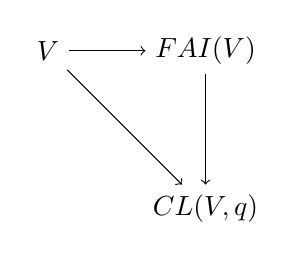
\begin{tikzpicture}[node distance=2cm, auto]
    \node (V) {$V$};
    \node (FAI) [right of= V] {$FAI(V)$};
    \node (CL) [below of= FAI] {$CL(V,q)$};
    \draw[->] (V) to (FAI);% corrected here
    \draw[->] (FAI) to (CL);% here
    \draw[->] (V) to (CL);% and here
    \end{tikzpicture}$$

    
    \item Un conjunto $A \subset \mathbb{R}^n$ es llamado convexo cuando para cualquier par de puntos $a, b \in A$ el segmento $[a,b] = \{ a + t(b-a): t \in [0,1] \}$ está contenido en $A$. Demuestre que las bolas definidas por cualquier norma son convexas.
    \item Demuestre que la conexidad por caminos es un invariante topológico.
    \item Demuestre que el determinante $\det: \mathbb{R}^{n^2} \to \mathbb{R}$ es una función continua.
    \item Demuestre que $GL(n, \mathbb{R})$ es un abierto denso de $\mathbb{R}^n$.
    \item Demuestre que cualquier esféra $S[a, r] \subset \mathbb{R}^n$ es conexa por caminos. Concluya que todas las esféras son conexas.
    \item Una aplicación $f:A \to B$ se dice abierta cuando la imagen de todo abierto en $A$ es abierto en $B$. Demuestre que si $f:X \to \mathbb{S}^n$ con $X$ compacto es abierta, entonces es sobreyectiva.
    \item La envolvente convexa de un conjunto $A \subset \mathbb{R}^n$ se define como la intersección de todos los convexos que contienen a $A$. Demuestre que la envolvente convexa de $A$ es igual al conjunto de todas las combinaciones lineales convexas de elementos de $A$, donde por combinación lineal convexa se entiende $\sum_{i=1}^k \alpha_i a_i$, $a_i \in A$, $\alpha_i \in [0,1]$ y $\sum \alpha_i = 1$. 
    \item Demuestre que para cualquier par de matrices $A, B \in \mathbb{R}^{n^2}$ se cumple $\det (I + AB) = \det (I + BA)$.
    \item Sea $f: \mathbb{R}^n \to \mathbb{R}$ con las siguientes dos propiedades. Para cualquier $a,b \in \mathbb{R}^2$ se cumple que la función $t \mapsto f(a + tv)$ es continua. Para cada compacto $K \subset \mathbb{R}^2$ se cumple que $f(K)$ es un compacto de la recta. Demuestre que $f$ es continua.
\end{enumerate}


\end{section}
\end{chapter}
